\documentclass{llncs}
\usepackage{times}
\usepackage[portuguese]{babel}
\usepackage[utf8]{inputenc}
\usepackage[T1]{fontenc}

% Comentar para not MAC Users
% \usepackage[applemac]{inputenc}

\usepackage{a4}
%\usepackage[margin=3cm,nohead]{geometry}
\usepackage{epstopdf}
\usepackage{graphicx}
\usepackage{fancyvrb}
\usepackage{amsmath}
\usepackage{float}
\usepackage{indentfirst}
%\renewcommand{\baselinestretch}{1.5}

\begin{document}

\title{Relatório TP2}
\titlerunning{Relatório TP2}
\author{Carlos Silva, João Coelho e Miguel Silva}
\authorrunning{Carlos Silva, João Coelho e Miguel Silva}

\institute{
Universidade do Minho, Departamento de Informática, 4710-057 Braga, Portugal\\
e-mail: \{a75107,a74859,a74601\}@alunos.uminho.pt
}

%\para não aparecer data
\date{}
\bibliographystyle{splncs}

\maketitle

\begin{abstract}
Rabanadas
\end{abstract}

\newpage

\section{Introdução}

\subsection{Contextualização}

Em muitos serviços Web, um único servidor não é suficiente para dar vazão aos pedidos dos clientes. Nesses casos, é necessário ter uma pool de N servidores de back-end, capazes de dar resposta aos pedidos. Ainda assim, o serviço terá um único ponto de entrada, comum a todos os
clientes, que se trata de um servidor de front-end, com nome e endereço IP únicos e bem conhecidos. A tarefa deste servidor, habitualmente designado por \textit{Reverse Proxy}, é atender as conexões dos clientes e desviá-las para um dos servidores de back-end disponíveis.\par
A escolha do servidor pode ser cega, baseada por exemplo num algoritmo de Round-Robin, que faz uma distribuição equitativa das conexões pelos N servidores de back-end, mas será esta a melhor solução?

\subsection{Exposição do problema}

O principal objetivo deste trabalho é desenhar e implementar um serviço simples de proxy reverso TCP, em que a escolha do servidor a usar se
faz com base em parâmetros dinâmicos, como por exemplo o RTT, as perdas e número de conexões TCP do servidor. Para tal, é necessário haver monitorização dos dados do estado do servidor e da rede, redirecionando em função de uma métrica dinâmica bem definida. Pretende-se desenhar e implementar um protótipo simples desta abordagem, separando-a em dois momentos: numa primeira fase temos um protocolo sobre UDP, para criar e manter atualizada uma tabela com dados recolhidos por agentes de monitorização; depois, numa segunda fase, pretende-se implementar um servidor proxy TCP genérico, que fique à escuta na porta 80 e redirecione, automaticamente, cada conexão TCP que recebe para a porta 80 de um dos servidores de back-end disponíveis (o que aparente estar em melhores condições para o fazer).

\begin{figure}[H]
\centering
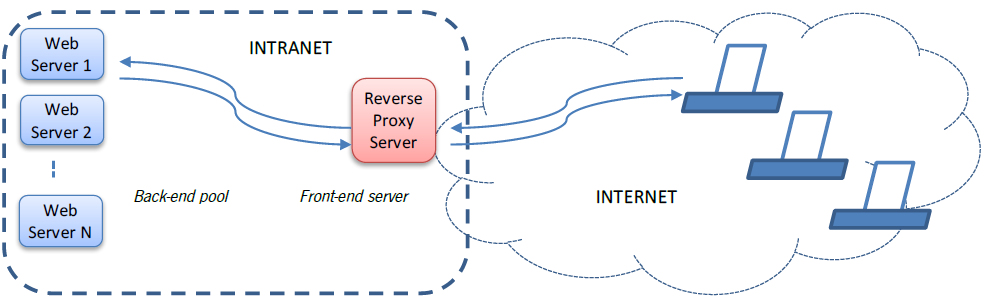
\includegraphics[width=150mm, scale=0.5]{imagem_enunciado.PNG}
\caption{\label{fig:change}Esquematização da arquitetura do problema.}
\end{figure}

\newpage

\section{Arquitetura da solução implementada}
-------------		  --------------\par
|  Back-end |		  |            |\par
|     (5555)|---------|            |\par
|  apache2  |		  |            |\par
-------------		  |            |\par
					  |Reverse (80)|-------- Clientes (wget)\par
-------------		  |	Proxy      |\par
|  Back-end |		  |            |\par
|     (5555)|---------|(5555)      |\par
|  apache2  |		  |            |\par
-------------		  --------------\par

\newpage

\section{Especificação do protocolo de monitorização}

\begin{itemize}
	\setlength\itemsep{1em}
\item \textbf{Primitivas de comunicação:} Carrega Benfica
\item \textbf{Formato do PDU:} constituído pelo número do ACK do próximo pacote, que o servidor pretende receber, e pelo timestamp que permitirá calcular o RTT. Sobre o ACK, importa referir que é utilizado no cálculo do taxa de perdas e de duplicados. Já sobre o timestamp, nota para o cuidado especial que se teve para que contabilizasse apenas o tempo de deslocamento de um pacote entre servidores. Aquando da receção de um pacote, o monitor marca o momento. A esse valor temporal subtrai o timestamp recebido, obtendo assim o tempo da deslocação até si. Depois, no momento em que se prepara para enviar a resposta ao pedido de probing, volta a calcular o tempo atual, subtraindo o valor do tempo da deslocação. Assim, ao receber a resposta, o Reverse Proxy só tem de calcular o momento atual e subtrair o timestamp recebido na resposta, obtendo assim o RTT.
\item \textbf{Interações:} Hellos de 5 em 5 segundos, com pedidos de probing smp que recebemos um estou disponivel
\end{itemize}

\newpage

\section{Implementação}

detalhes, parâmetros, bibliotecas de funções, etc.

\newpage

\section{Testes e resultados}

Usamos apache2 blah blah

\newpage

\section{Conclusões e trabalho futuro}

No futuro não quero mais disto

\newpage
%UNCOMMENT para a bibliografia 
%% ficheirodebibliografia.bib
%\bibliography{ficheirodebibliografia}

%ou inserir directamente os v‡rios \bibitem 
\begin{thebibliography}{1}

%Exemplo de notaçao
%\bibitem{Figura 1}
%Figura 1:
%\newblock {http://i1.wp.com/mammothgamers.com/wp-content/uploads/2016/07/FullSizeRender.jpg} (2016)

%\bibitem{Figura 2}
%Figura 2:
%\newblock {https://i.ytimg.com/vi/RjMS15V\textunderscore 7nQ/maxresdefault.jpg} (2016)

%\bibitem{Edge1}
%Mixon, E.: edge computing (2016)

%\noindent http://searchdatacenter.techtarget.com/definition/edge-computing

\end{thebibliography}

\end{document}